\subsubsection{No Optimizations (\texttt{-O0})}

We begin by compiling the baseline implementation with the \texttt{-O0} flag, which disables virtually all compiler optimizations. This configuration isolates the raw, intrinsic computational and memory access characteristics of the algorithm without interference from auto-vectorization or loop restructuring. 

\begin{figure}[H]
  \centering
  \noindent
  \makebox[0pt][c]{%
    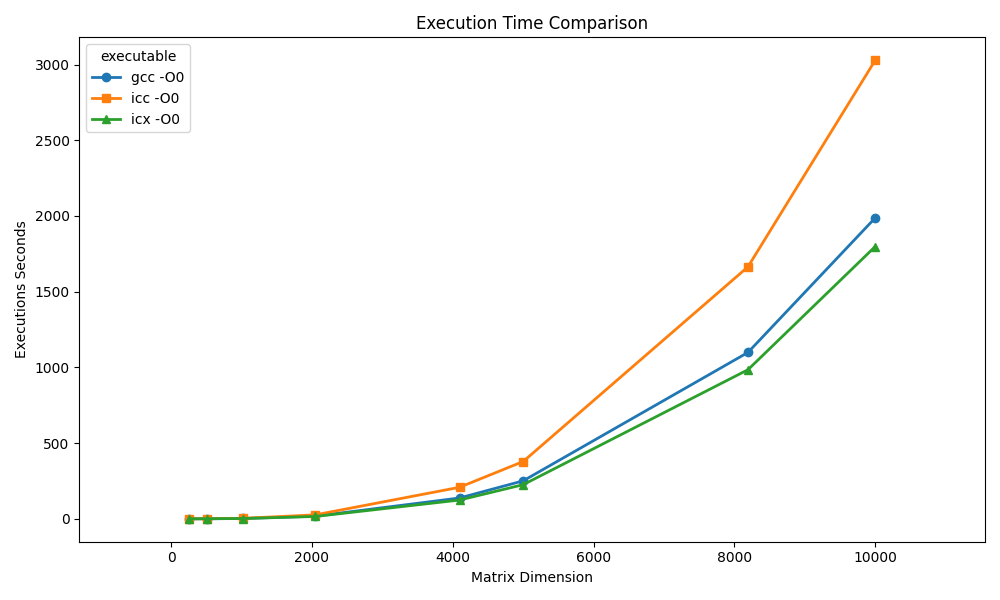
\includegraphics[width=0.6\paperwidth]{Images/all_o0.png}
  }
  \caption{Execution time scaling as a function of matrix size ($n$) at \texttt{-O0}.}
  \label{fig:all_o0}
\end{figure}

\paragraph{Performance Scaling.}
Figure~\ref{fig:all_o0} reports the execution time as a function of matrix size $n$ for the three compilers at \texttt{-O0}. Across all tested input sizes, the scaling behavior strictly follows the expected cubic trend $\mathcal{O}(n^3)$, confirming the theoretical complexity of the algorithm. At this level performance is severely limited, and significant discrepancies observed among the compilers, are not interesting to address, since the generated machine code is a literal, unoptimized translation of the source code.


\paragraph{Intel Advisor and Roofline Analysis.}

The Roofline model (Figure~\ref{fig:icc_o0_roofline}) places the kernel at an extremely low arithmetic intensity ($\approx 0.014$ FLOP/Byte) with a measured performance of merely \textbf{0.66 GFLOPS}. 
Crucially, Advisor indicates that the execution is bottlenecked by the \textbf{Integer Scalar Add Peak} rather than floating-point throughput or memory bandwidth.

\begin{figure}[H]
\centering
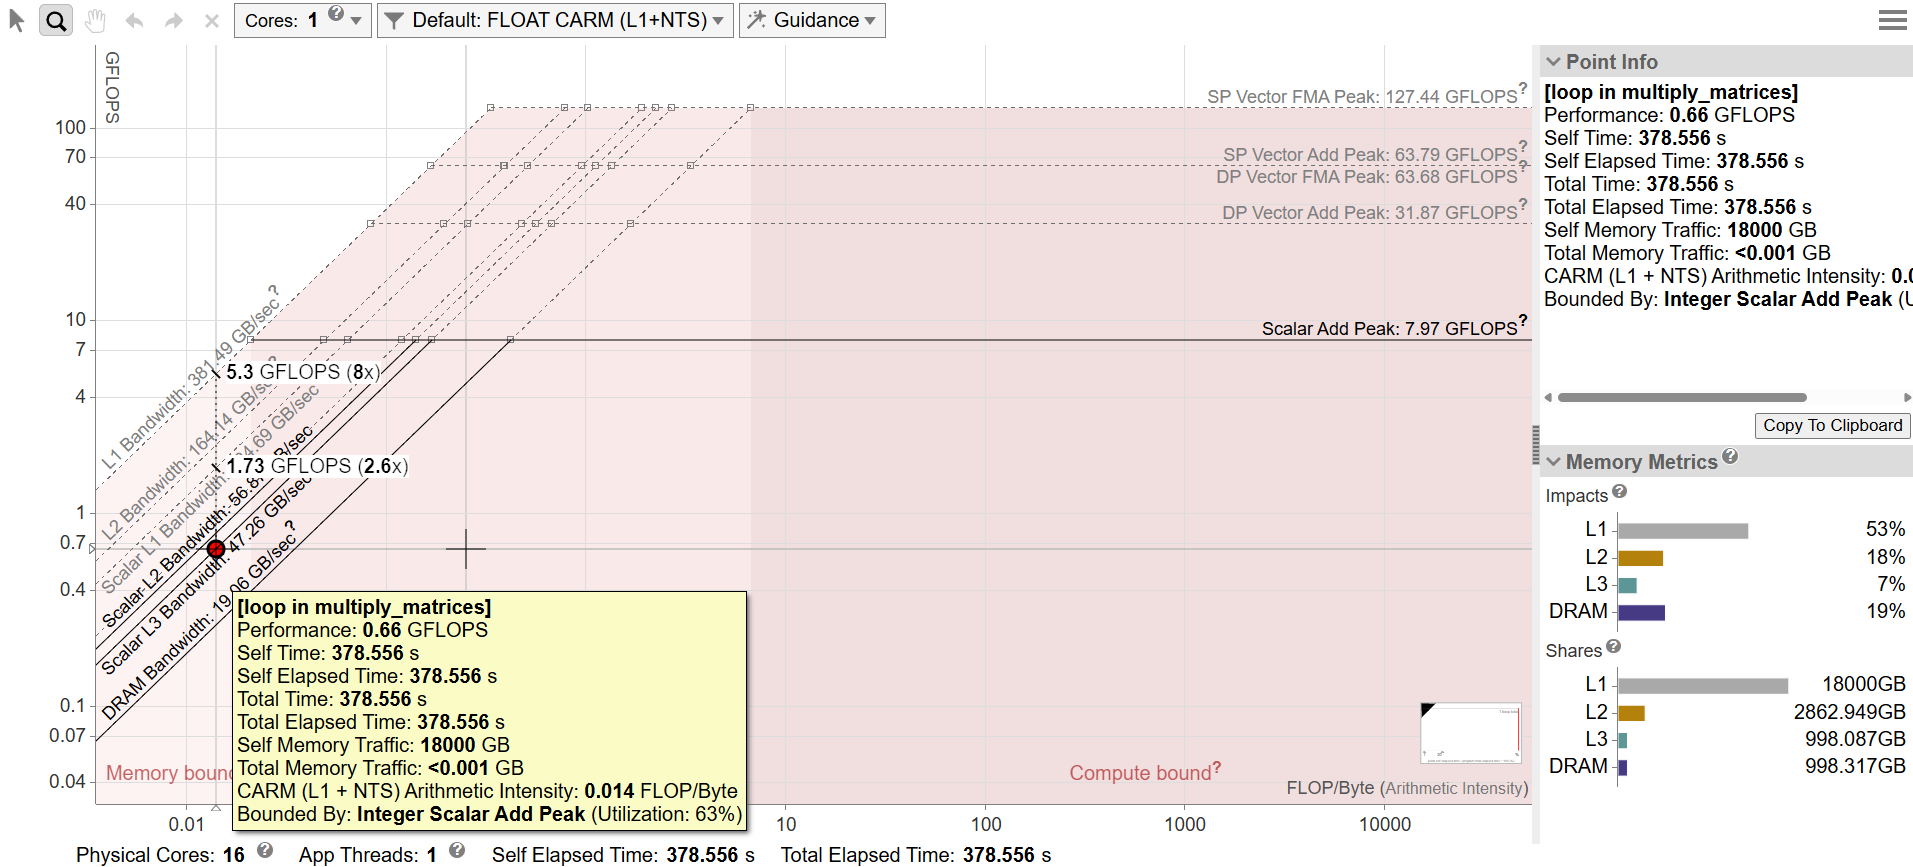
\includegraphics[width=1\textwidth]{Images/icc_o0_roofline.png}
\caption{Intel Advisor Roofline analysis for ICC \texttt{-O0}.}
\label{fig:icc_o0_roofline}
\end{figure}

This massive integer overhead is a direct consequence of the address calculation required for every 2D array access\footnote{The standard 2D array syntax implicitly expands the logical coordinates \texttt{A[i][j]} into a offset \texttt{A[i * n + j]}, requiring a scalar integer multiplication and addition for every single element accessed.}.

Under \texttt{-O0}, the compiler does not perform common subexpression elimination, strength reduction, or loop-invariant code motion. Consequently, these redundant index multiplications and additions are re-evaluated during every single iteration of the innermost loop. Furthermore, the strict lack of register allocation forces the CPU to continuously spill and reload these intermediate address calculations to and from the L1 cache, completely stalling the floating-point pipelines\footnote{This it the main cause of the slow-down, as confirmed by the extremely high number of requests to the L1 cache.}.


\paragraph{Valgrind Cachegrind Analysis.}
The excessive memory traffic caused by the lack of register reuse is confirmed by Valgrind (Figure~\ref{tab:cachegrind_results_o0}). 

\begin{table}[H]
\centering
\caption{Key Valgrind Cachegrind memory profiling metrics for ICC \texttt{-O0}.}
\label{tab:cachegrind_results_o0}
\begin{tabular}{lr}
\toprule
\textbf{Metric} & \textbf{Total Count / Rate} \\
\midrule
Instruction References (I) & \textbf{6,626,402,614,521} \\
Data References (D)        & \textbf{3,000,701,173,012} \\
\midrule
L1 Data Misses             & 31,287,508,170 \\
L1 Data Miss Rate          & 1.0\% \\
\midrule
Last-Level (LL) Misses     & 15,640,639,539 \\
Last-Level (LL) Miss Rate  & 0.2\% \\
\bottomrule
\end{tabular}
\end{table}

The profiling reports approximately 6.6 trillion executed instructions (I refs) alongside 3 trillion data references (D refs). This ratio of roughly 2.2 instructions per data access reflects the massive scalar overhead required simply for loop control and address calculation. 

Despite an enormous cumulative memory traffic footprint ($\approx 18$ TB of L1 interactions), the actual cache miss rates remain relatively low (1.0\% for L1 data, 0.2\% for Last-Level Cache). This confirms that the kernel is not DRAM bandwidth-bound, but rather instruction-bound due to scalar execution.


\paragraph{Compiler Report.}
Finally, the compiler optimization report for \texttt{-O0} confirms the absence of any code transformations. No SIMD instructions are generated (the code relies exclusively on standard scalar x86 instructions), and the nested loops are left entirely intact without unrolling, blocking, or interchange, leading to the severe underutilization of the CPU's computational resources observed in the profiling tools.